\vspace{-3cm}\chapter{实验6. 蒙特·卡洛方法模拟}

\section{6.1 题目}

编写一个程序来模拟蒙特卡罗方法。具体的过程可以按照下面的方式来模拟:如下图所示(a)中的正方形,假设向正方形
所代表的区域投掷飞镖,如果投掷100000次,那么飞镖落在奇数数字所对应区域的概率是多少呢? 

\begin{figure}[H]
    \centering
    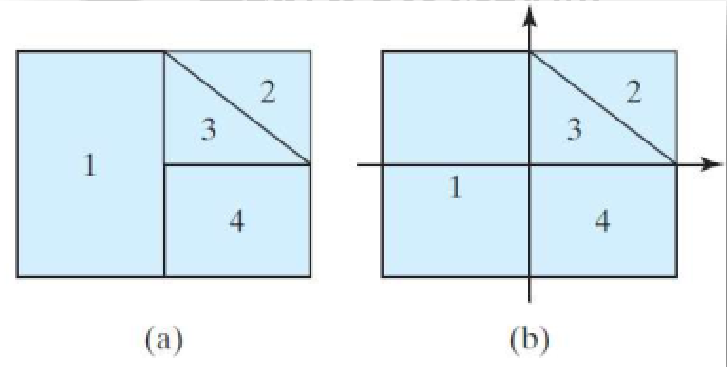
\includegraphics[width = 0.8\textwidth]{../pic/6/6.0.png}
\end{figure}

提示:可以将(a)图放到如(b)所展示的坐标系中,程序随机的在整个区域中生成点,这样模拟投掷飞镖的行为。

\section{6.2 思路分析}
\begin{enumerate}
    \item 如题目中提示所说,可以如b图所示建立坐标系,程序随机地在区域中生成点(即生成两个范围内的数作为横纵坐标)
    \item 为了模拟更精确,随机生成
        应该采用\lstinline[language = Java]{double nextDouble(double origin, double bound)}随机生成小数。
        代码中设正方形的范围为$[-100,100]\times[-100,100]$。
    \item 每次生成后需要判断该点是否在奇数数字,即1、3区域,通过简单的平面几何相关知识即可确定。如果在就将用来记录次数的变量+1。
    \item 随机生成100000次结束后输出记录次数的变量/100000的值,此处需要注意的是需要强制转换为double否则会自动转为整型。
\end{enumerate}

\section{6.3 代码与结果展示}

代码如下

\lstinputlisting[
    language = Java,
    caption = {\bf Problem6.java}
]{../../../ProblemSet/src/Problem6.java}

结果如下

\begin{figure}[H]
    \centering
    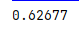
\includegraphics[width = 0.15\textwidth]{../pic/6/6.1.png}    
\end{figure}

\section{6.3 总结与收获}

本题看似简单但输出有一个大坑,即强制转换,很久没使用我几乎已经遗忘了这个性质

本题的名字看似唬人,但题目难度很低,不要被吓到,仔细阅读要求即可